% Auto-generated by scripts/build_ch5_evidence_tables.py (final drafting pass, 2026-10).
\begin{figure}[!htbp]
\centering
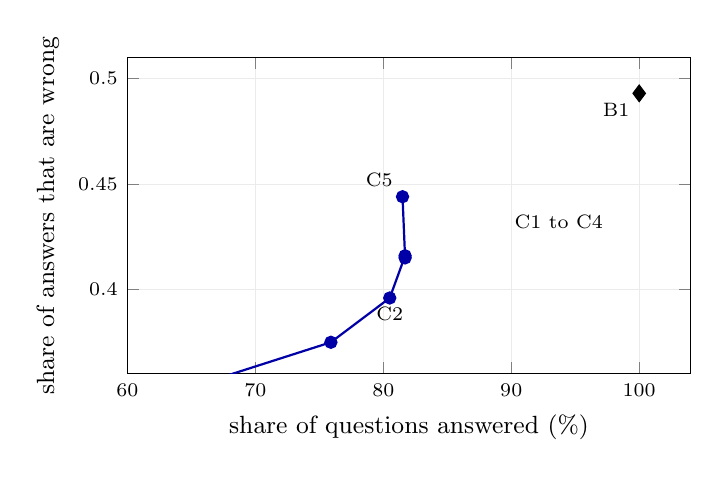
\begin{tikzpicture}
\begin{axis}[width=0.72\textwidth, height=5.6cm, xlabel={share of questions answered (\%)}, ylabel={share of answers that are wrong},
  xmin=60, xmax=104, ymin=0.36, ymax=0.51, font=\small, tick label style={font=\scriptsize}, grid=major, grid style={black!8}]
  \addplot[blue!65!black, mark=*, thick] coordinates {(34.2,0.294) (75.9,0.375) (80.5,0.396) (81.7,0.416) (81.7,0.415) (81.5,0.444)};
  \node[font=\scriptsize, anchor=south east] at (axis cs:34.2,0.294) {C0};
  \node[font=\scriptsize, anchor=north] at (axis cs:80.5,0.396) {C2};
  \node[font=\scriptsize, anchor=south east] at (axis cs:81.5,0.444) {C5};
  \node[font=\scriptsize, anchor=west] at (axis cs:89.5,0.432) {C1 to C4};
  \addplot[black, only marks, mark=diamond*, mark size=3pt] coordinates {(100,0.493)};
  \node[font=\scriptsize, anchor=north east] at (axis cs:100,0.493) {B1};
\end{axis}
\end{tikzpicture}
\caption[Answered share against error among answered.]{Selective-prediction view on the evaluation fold: share of questions answered and share of those answers that are wrong, for each cycle and for B1, which answers everything. CAEM stays below B1's error but answers more and errs more as the cycles go on.}
\label{fig:selective}
\end{figure}
